\documentclass[border=1pt]{standalone}
\usepackage[dvipsnames]{xcolor}
\usepackage{tikz}                       % Graphen und kommutative Diagramme
\usetikzlibrary{patterns}               % Um schraffierte Formen in der tikzpicture-Umgebung zu zeichnen.


\begin{document}
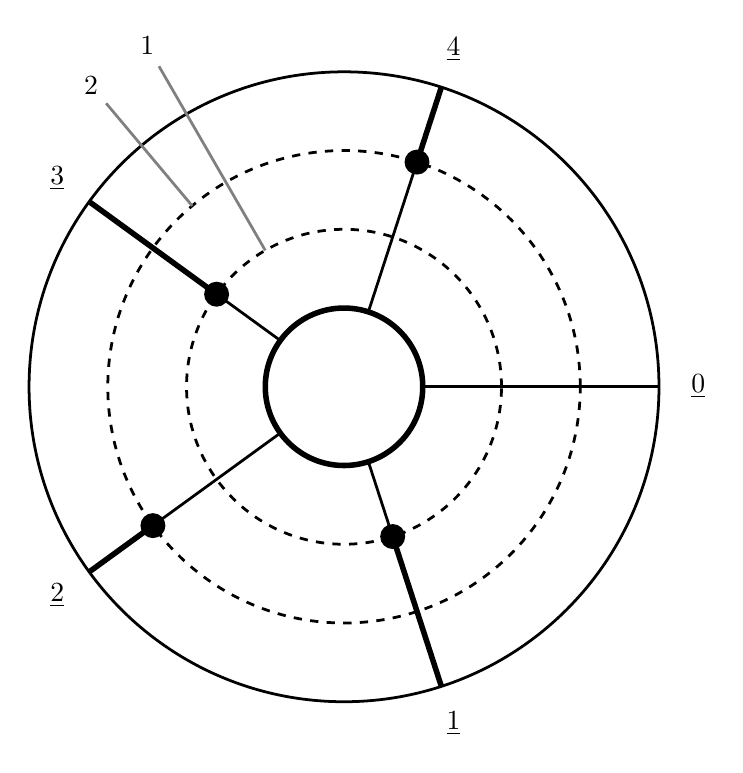
\begin{tikzpicture}[line width=1pt]

\newcommand{\ul}{\underline}

% draw inner and outer circles
\draw[color=black, line width=2pt] (0, 0) circle (1);
\draw[color=black] (0, 0) circle (4);

% draw dashed circles
\foreach \i in {2,...,3}
{
    \draw[color=black, dashed] (0, 0) circle (\i);
}

% draw radial segment
\foreach \i in {0,...,4}
{
		\draw (\i * 72 : 1) -- (\i * 72 : 4);
}

% label the slits
\foreach \i in {0,...,4}
{
		\draw node at (72 * 4 * \i : 4.5) {\ul \i};
}

% label the concentrical lines
\draw node at (120 : 5) {$1$};
\draw[color=black!50] (120 : 4.7) -- (120 : 2);
\draw node at (130 : 5) {$2$};
\draw[color=black!50] (130 : 4.7) -- (130 : 3);

% draw slits
\draw[color=black, line width=2pt] (72 : 3) -- (72 : 4);
\draw[color=black, line width=2pt] (2*72 : 2) -- (2*72 : 4);
\draw[color=black, line width=2pt] (3*72 : 3) -- (3*72 : 4);
\draw[color=black, line width=2pt] (4*72 : 2) -- (4*72 : 4);
\filldraw (72 : 3) circle (4pt);
\filldraw (2*72 : 2) circle (4pt);
\filldraw (3*72 : 3) circle (4pt);
\filldraw (4*72 : 2) circle (4pt);

\end{tikzpicture}
\end{document}